\documentclass[a4paper,10pt]{article}
\usepackage[utf8]{inputenc}
\usepackage[T1]{fontenc}
\usepackage[english]{babel}
\usepackage{times}
\usepackage{graphicx}
\usepackage{tikz}
\usepackage{circuitikz}
\textwidth=6in
\textheight=9.0in
\headheight=0in
\headsep=0in
\oddsidemargin=0in
\evensidemargin=0in
\title{SSM2164 4-pole with pole-mixing}
\author{Olivier Gillet -- \tt ol.gillet@gmail.com}
\date{}
\begin{document}

\maketitle

This document explains the inner workings of the ``Pole mixer" filter board, which uses a SSM2164 4-pole core along with a pole-mixer to realize 15 different transfer functions.

\section{VCA-based 1-pole LPF}

We remind here that a SSM2164 VCA cell works as a voltage-controlled current attenuator, according to the following equation:

$$i_{out} = i_{in} 10^{-\frac{3}{2} v_c}$$

Note that input pin of the SSM2164 is part of a differential pair whose other input is internally grounded (please refer to figure 23 in the SSM2164 datasheet), so the input pin is at ground potential and $i_{in}$ is simply $\frac{v_{in}}{R}$.

Let us model the circuit in figure \ref{fig:vcf} from left to right. The current at the input of the VCA is the sum of the input current, and the current fed back from the output:

\begin{figure}
\begin{center}
\begin{circuitikz} \ctikzset{bipoles/not port/circle width=0}
 \draw
 (0, 0) node[op amp] (opamp) {}
 (opamp.-) node[anchor=south] {$v'_-$}
 (opamp.+) to[short] (-1.5, -0.5)
 (opamp.out) to[short, -] (3, 0)
 (3, 0) node[anchor=south] {$v_o$}
 (-1.5, -0.5) to (-1.5, -1)
 (-1.5, -1) node[ground] {}
 (opamp.-) to[, -*] (-1.5, 0.5)
 (-1.5, 0.5) to (-1.5, 1.5)
 (-1.5, 1.5) to[C, C=$C$, -*] (2, 1.5)
 (2, 1.5) to[short] (2, 0)
 (2, 0) to[*-] (opamp.out)
 (2, 1.5) to (2, 3)
 (2, 3) to[R, R=$R$] (-4.5, 3)
 (-7, 0.5) to[R, R=$R$, i=$i_s$] (-5, 0.5)
 (-5, 0.5) to[short] (-4.5, 0.5)
 (-4.5, 3) to[i=$i_o$, -*] (-4.5, 0.5)
 (-3, 0.5) node[not port] (amp) {}
 (-4.5, 0.5) to[i=$i_{in}$] (amp.in)
 (amp.out) to[i=$i_{out}$] (-1.5, 0.5)
 (-7, 0.5) node[anchor=south] {$v_s$}
 (-3, -1) node[anchor=north] {$v_c$}
 (-3, -1) to (-3, 0.2)
;\end{circuitikz}
\end{center}
\caption{1-pole voltage-controlled low-pass filter based on a VCA cell}
\label{fig:vcf}
\end{figure}

\begin{eqnarray*}
i_{in}(p) &=& i_s(p) + i_o(p) \\
i_{in}(p) &=& \frac{1}{R}(v_s(p) + v_o(p))
\end{eqnarray*}

The op-amp is used as a current to voltage converter (or \emph{transimpedance amplifier}), and is inverting:

\begin{eqnarray*}
v_o(p) &=& -Z_{feedback}(p) i_-(p) \\
v_o(p) &=& -\frac{1}{Cp} i_{out}(p) \\
v_o(p) &=& -\frac{1}{Cp} 10^{-\frac{3}{2} v_c} i_{in}(p) \\
v_o(p) &=& -\frac{1}{Cp} 10^{-\frac{3}{2} v_c} \frac{1}{R}(v_o(p) + v_s(p)) \\
v_o(p) &=& \frac{-\frac{1}{RCp} 10^{-\frac{3}{2} v_c}v_s(p)}{\left(1 + \frac{1}{RCp} 10^{-\frac{3}{2} v_c} \right)}
\end{eqnarray*}

We can now compute the transfert function:

\begin{eqnarray*}
H(p) &=& \frac{v_o(p)}{v_s(p)} \\
H(p) &=& \frac{-1}{1 + RC 10^{\frac{3}{2} v_c} p} \\
\end{eqnarray*}

This is the transfer function of an \textbf{inverting} 1-pole low-pass filter, with a pole at the frequency zeroing the denominator:

\begin{eqnarray*}
1 + RC 10^{\frac{3}{2} v_c} 2 \pi f_c &=& 0 \\
f_c &=& \frac{-1}{2 \pi RC} 10^{-\frac{3}{2} v_c}
\end{eqnarray*}

With $R = 33k\Omega$ (the datasheet suggests $R = 30k\Omega$ for the voltage to current conversion on the SSM2164 inputs), and $C = 220pF$, a frequency range of $22Hz$ to $22kHz$ can be obtained with $v_c$ varying from $2.0V$ to $0.0V$ (the circuit doing this scaling is a simple op-amp in inverter configuration, not detailed here).

In the rest of this document we use the scaled variable $s = RC 10^{\frac{3}{2} v_c} p$ to simplify the transfer function of this 1-pole cell into $\frac{-1}{1 + s}$.

A simple 4-pole filter can be built by chaining 4 1-pole cells. The resulting transfer function is thus $\frac{1}{(1 + s)^4}$.

\section{Pole-mixing}

Pole-mixing consists in mixing, with different gains, the output of each 1-pole cell of a 4-pole filter. Let us call $a, b, c, d$ the gains applied to the output of the first, second, third and fourth cells ; and let us assume that the amplifier doing the summing and amplification is inverting. The resulting transfer function will thus be:

$$H_{a, b, c, d}(s) = \frac{a}{1 + s} + \frac{-b}{(1 + s)^2} + \frac{c}{(1 + s)^3} + \frac{-d}{(1 + s)^4}$$

Notice the alternating signs. This is because our SSM2164 based 1-pole cell is inverting, and this is very helpful indeed as we will see later! A little digression about this: In other pole-mixing circuits such as that of the Oberheim Xpander, additional op-amp stages are needed to buffer the output of each stage, and then to invert the output of each odd stage, requiring up to 6 op-amps to be added to the circuit. Here, the inversion and low-impedance output is built-in the low-pass cell itself, and the only thing to add for the mixing are resistors feeding into the virtual ground of a summing op-amp!

This ``mixed" transfer function can be expanded into:

$$H_{a, b, c, d}(s) = \frac{a s^3 + 3as^2-3as + a - b s^2 - 2bs - b + cs +c - d}{(1 + s)^4}$$

Any 4th order transfer function with $(1 + s)^4$ as its denominator:

$$H_{x, y, z, t}(s) = \frac{x s^3 + y s^2 + z s + t}{(1 + s)^4}$$

can be implemented by pole mixing using the coefficients $a, b, c, d$ which are solutions of these linear equations:

$$\left\{\begin{array}{c}
a = x \\
3a - b = y \\ 
3a - 2b + c = z \\
a - b + c - d = t
\end{array}\right.$$

A bank of resistors behind (a) multiplexer(s) can be used to switch sets of $a, b, c, d$ coefficients. There are still a few problems with this solution though:

\begin{itemize}
\item It would require from 1 to 4 resistors per transfer function we want the filter to implement!
\item Transfer functions like $\frac{s}{1 + s}$ (1-pole HP) are not realizable with this system, since the order of the polynomial at the numerator can only be strictly lower than the order of the polynomial at the bottom.
\end{itemize}

A possible solution is to add a switch in the circuit to bypass the first low-pass cell (or more accurately use a lower integration cap to provide a very high cutoff-frequency). Using this approach, transfer functions of the form:

$$H_{x, y, z, t}(s) = \frac{x s^3 + y s^2 + z s + t}{(1 + s)^3}$$

can also be implemented using the same circuit and the same design equations, with the only change that the first inverting 1-pole cell has been bypassed and replaced by a simple inverting cell.

The second benefit of this ``switched first 1-pole" approach is that it is often the case that if $H(s)$ is an interesting transfer function, $H(s) (1 + s)$ will also be worth considering. Consequently, if a set of mixing resistors has been put in place for $H(s)$, it is trivial to just switch the first LP section off to realize $H(s) (1 + s)$.

\section{The 15 modes}

\subsection{Low-pass modes}

\begin{tabular}{lcclllll}
\hline
Name & Response & Transfer function & $a$ & $b$ & $c$ & $d$ & First LP stage \\
\hline
LP1 & 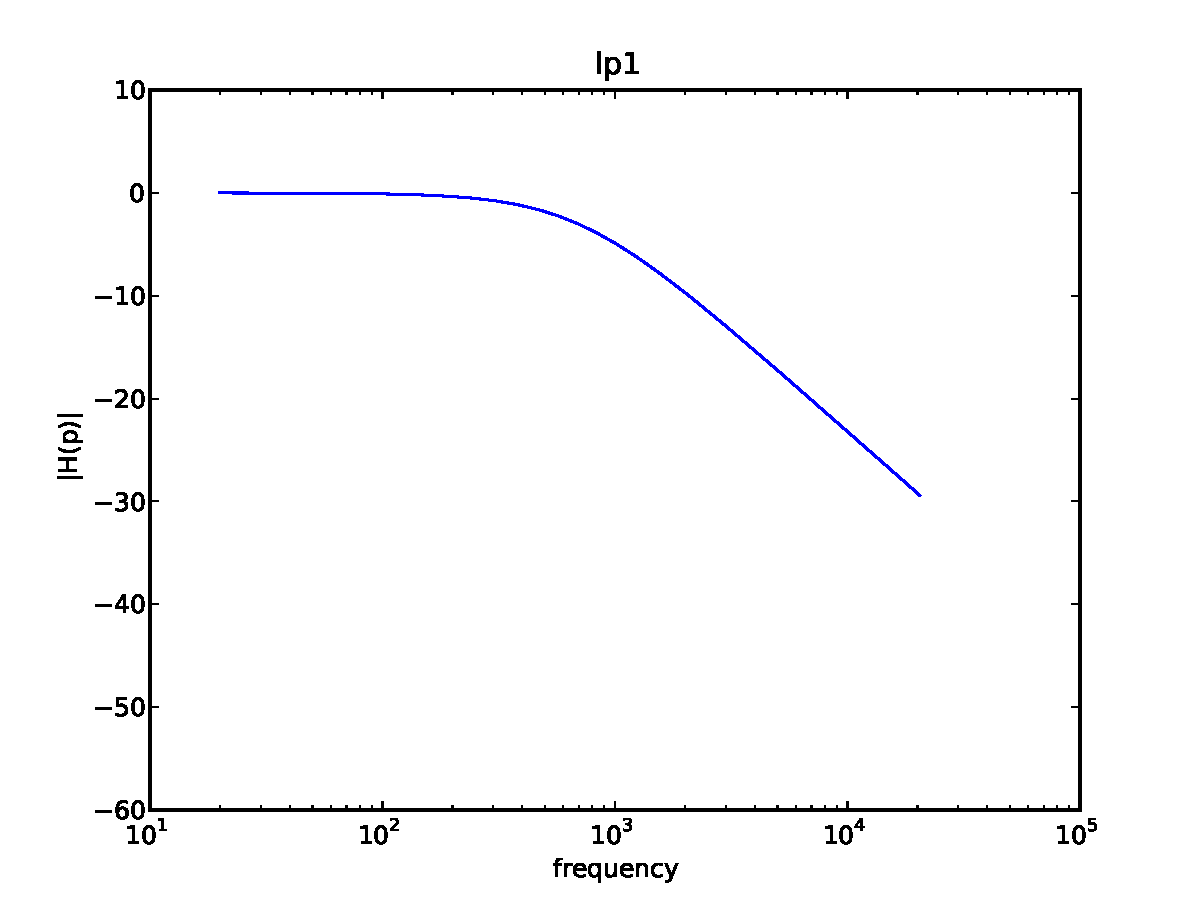
\includegraphics[width=0.4\textwidth]{response_lp1.pdf} & $\frac{1}{1 + s}$ & 0 & 1 & 0 & 0 & Disabled \\
\hline
LP2 & 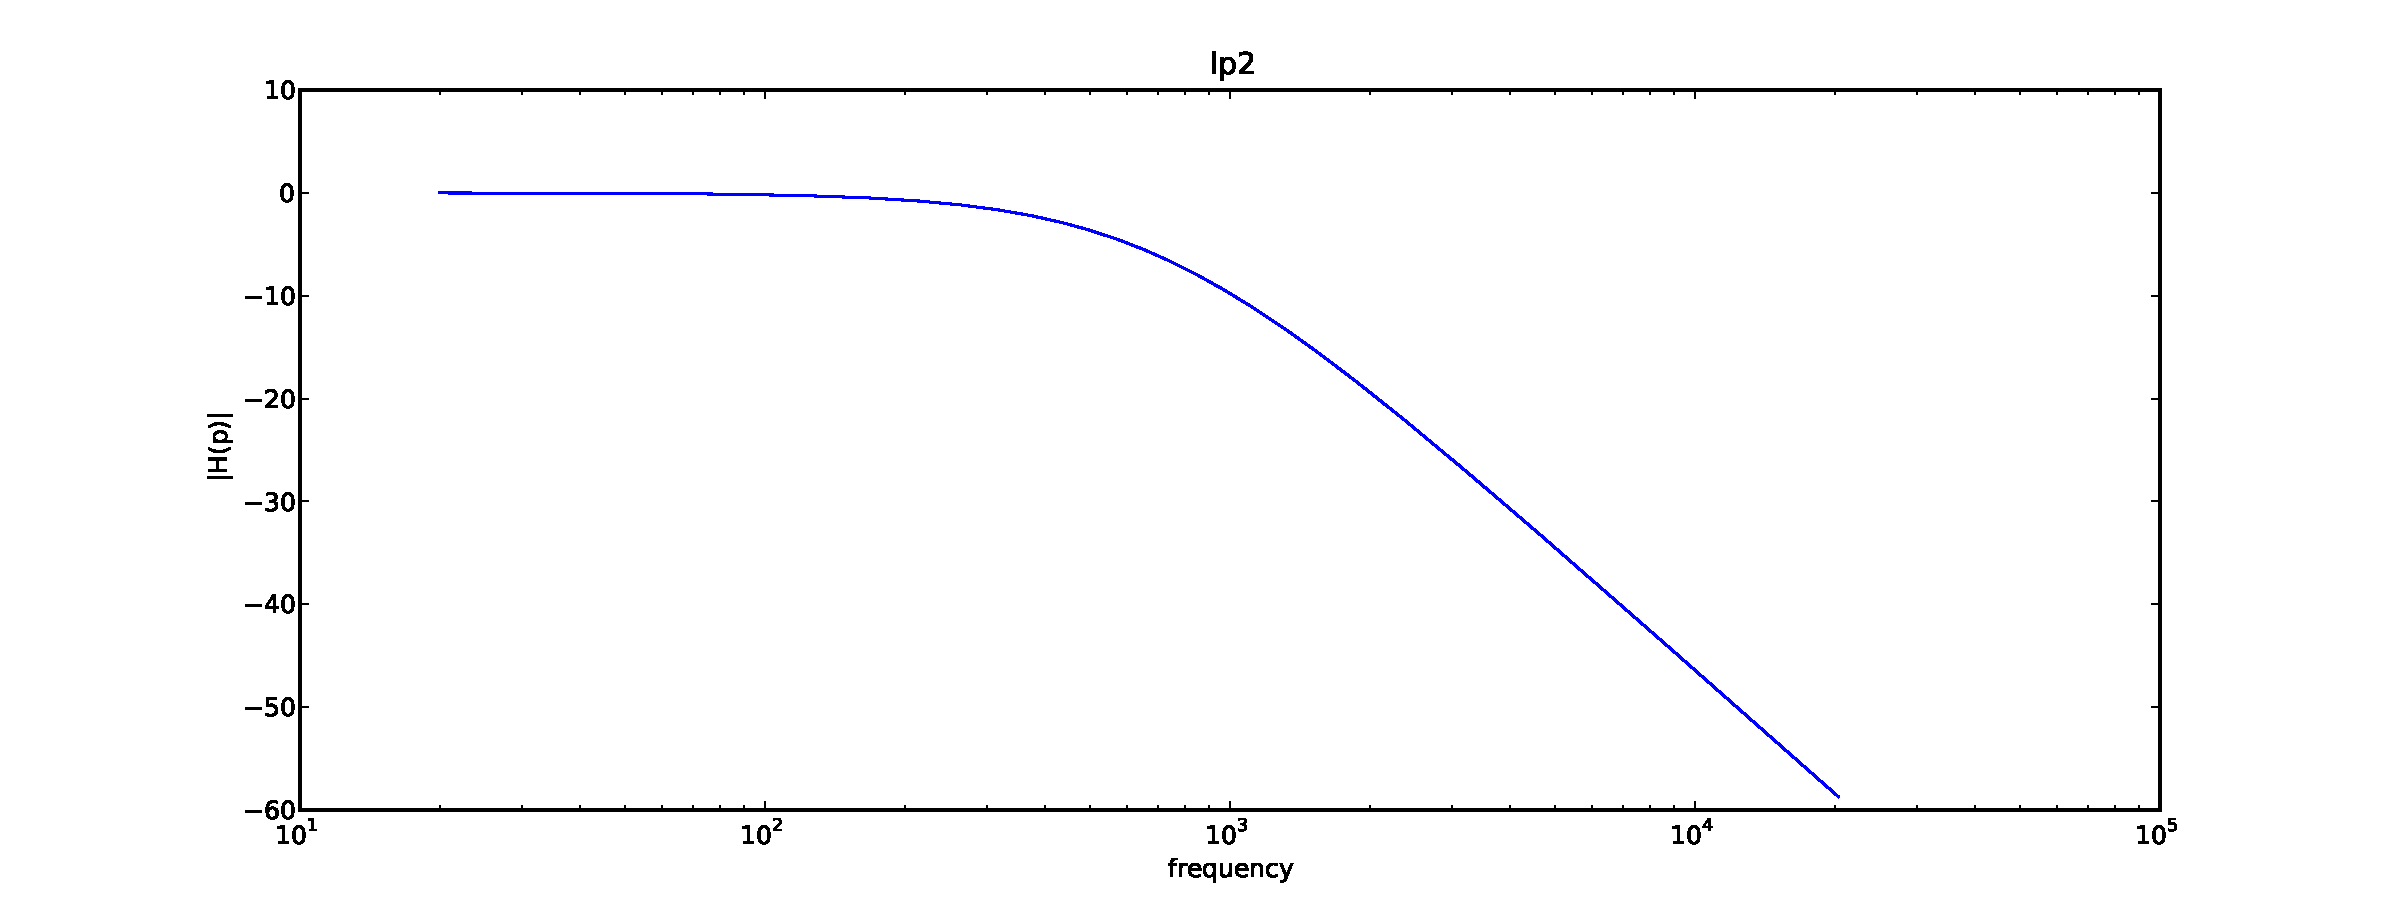
\includegraphics[width=0.4\textwidth]{response_lp2.pdf} & $\frac{1}{(1 + s)^2}$ & 0 & 1 & 0 & 0 & Enabled \\
\hline
LP3 & 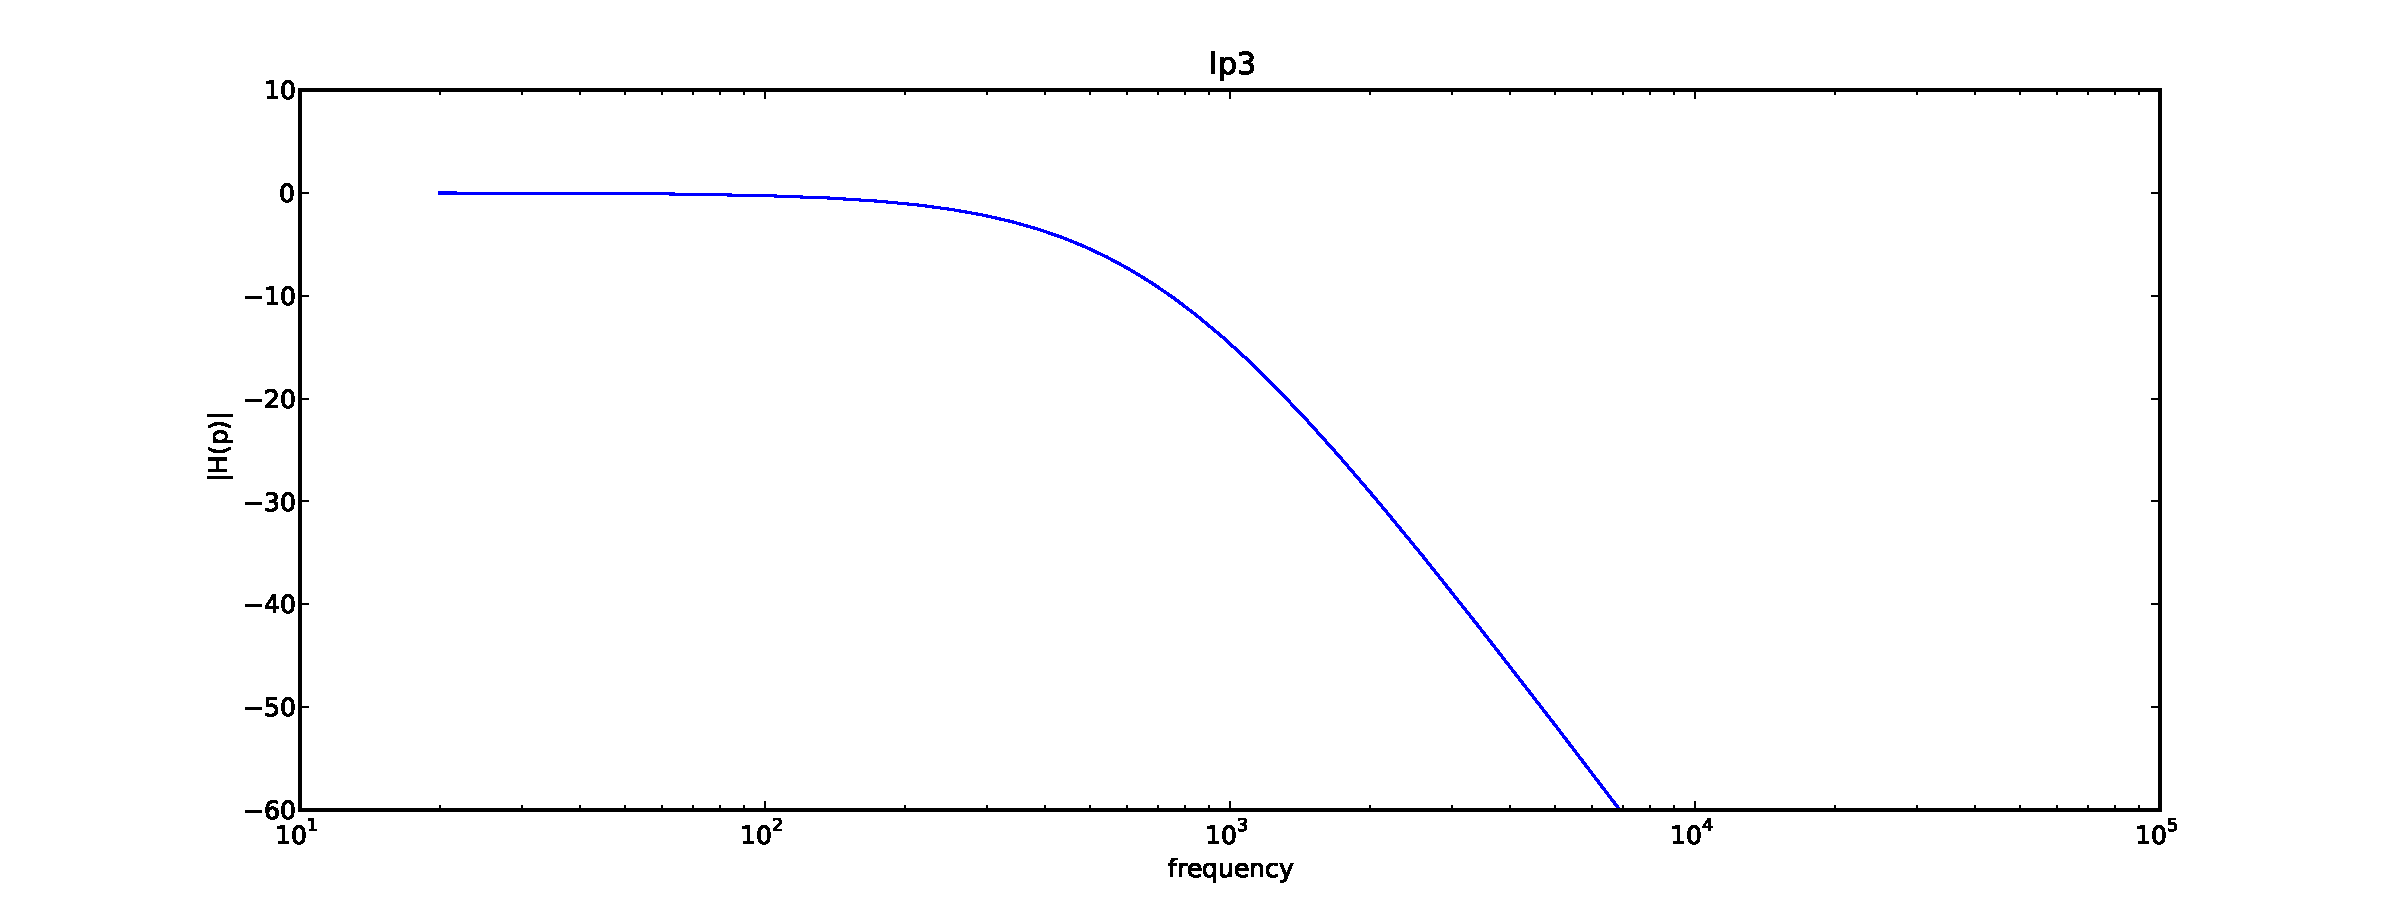
\includegraphics[width=0.4\textwidth]{response_lp3.pdf} & $\frac{1}{(1 + s)^3}$ & 0 & 0 & 0 & 1 & Disabled \\
\hline
LP4 & 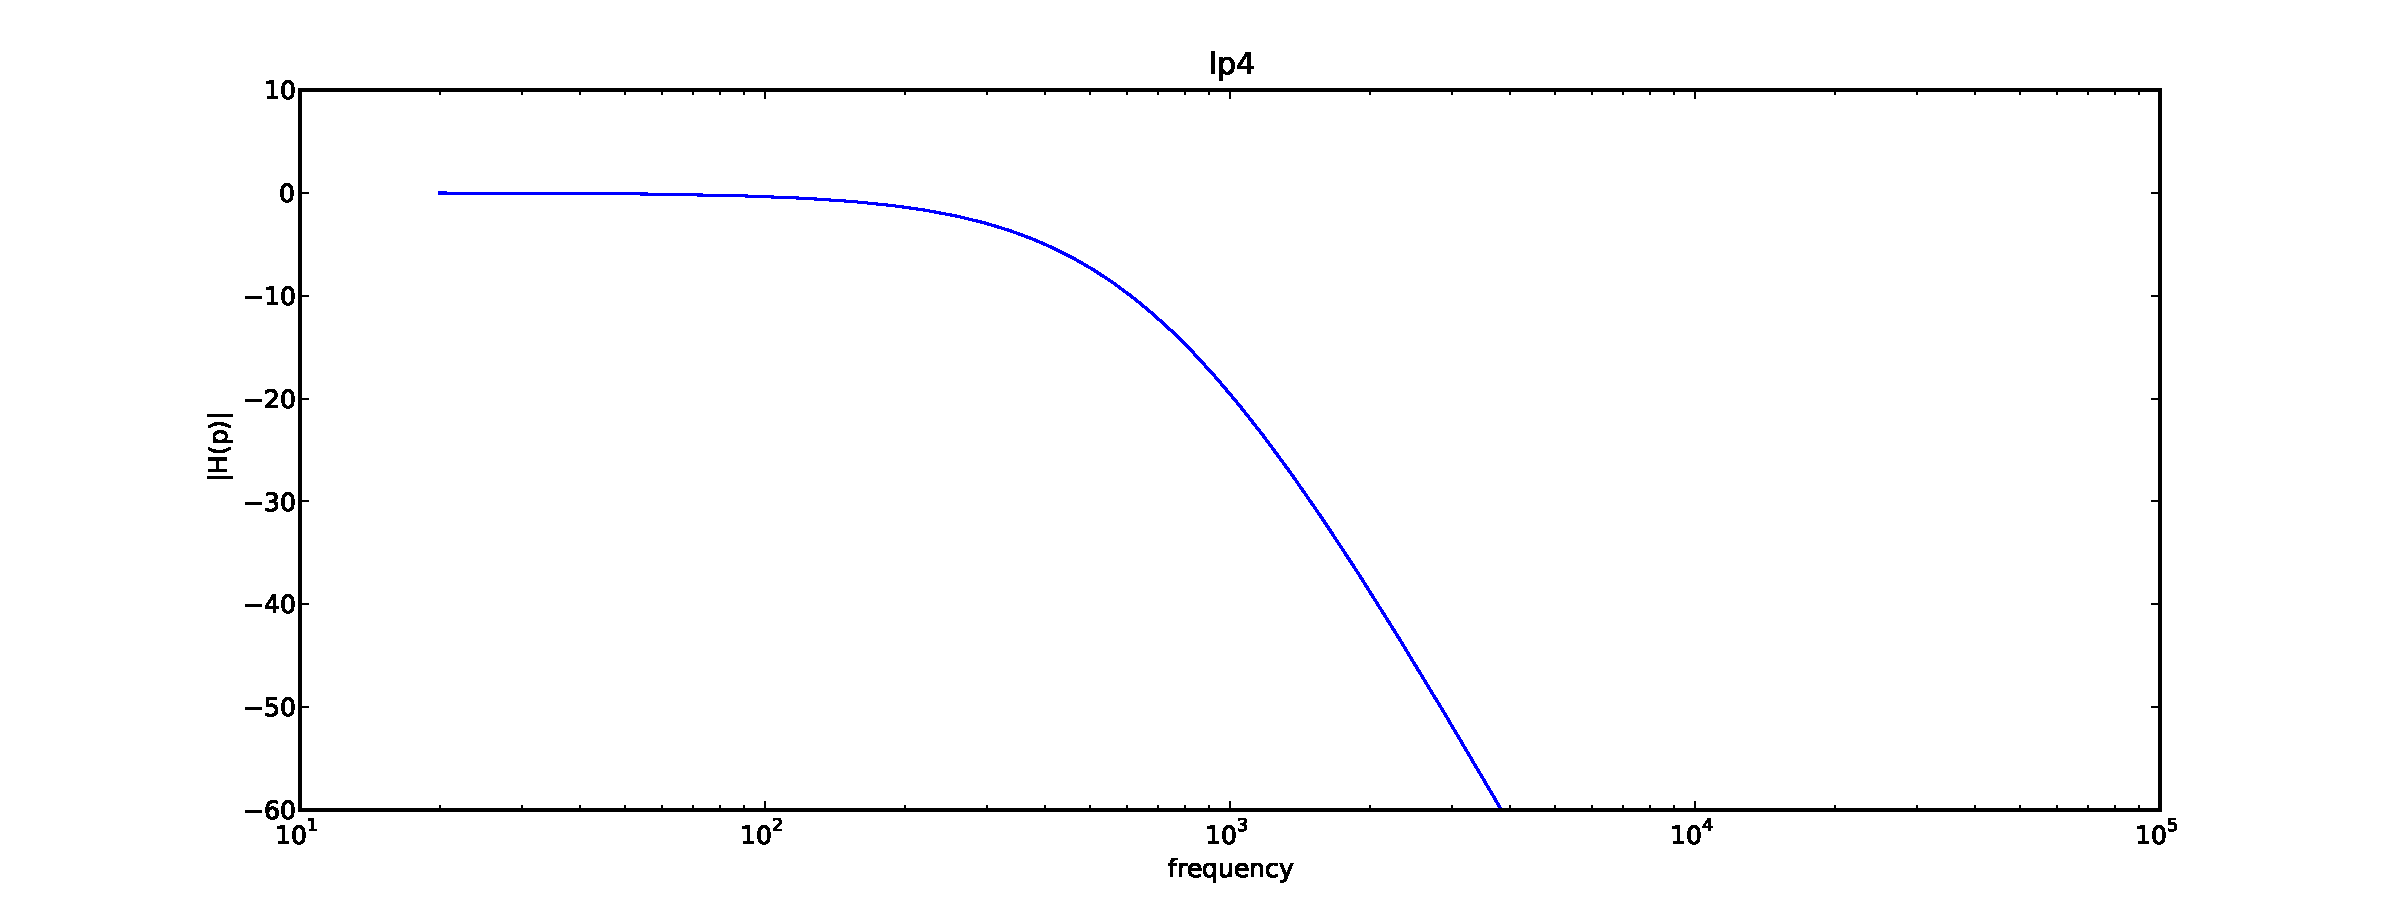
\includegraphics[width=0.4\textwidth]{response_lp4.pdf} & $\frac{1}{(1 + s)^4}$ & 0 & 0 & 0 & 1 & Enabled \\
\hline
\end{tabular}

\subsection{High-pass modes}

\begin{tabular}{lcclllll}
\hline
Name & Response & Transfer function & $a$ & $b$ & $c$ & $d$ & First LP stage \\
\hline
HP1 & 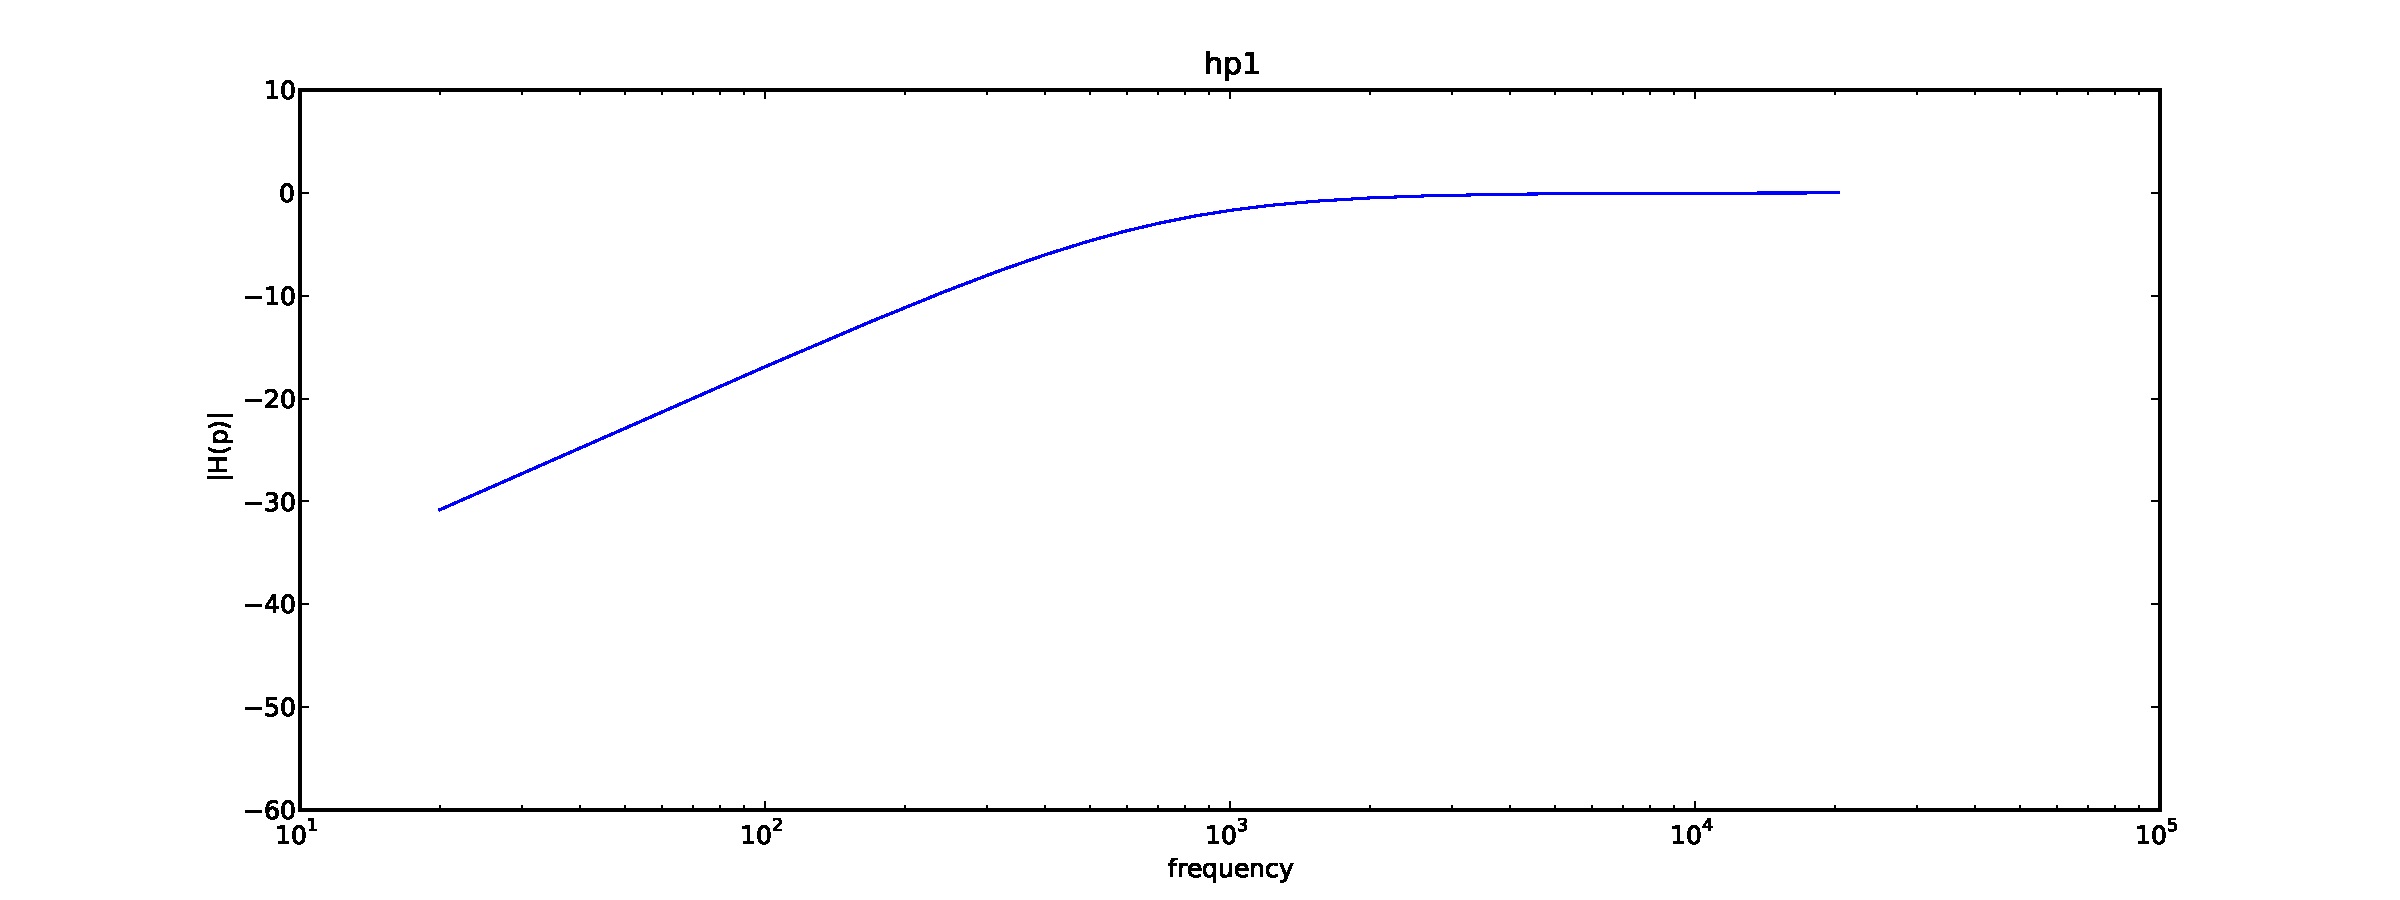
\includegraphics[width=0.4\textwidth]{response_hp1.pdf} & $\frac{s}{1 + s}$ & 1 & 1 & 0 & 0 & Disabled \\
\hline
HP2 & 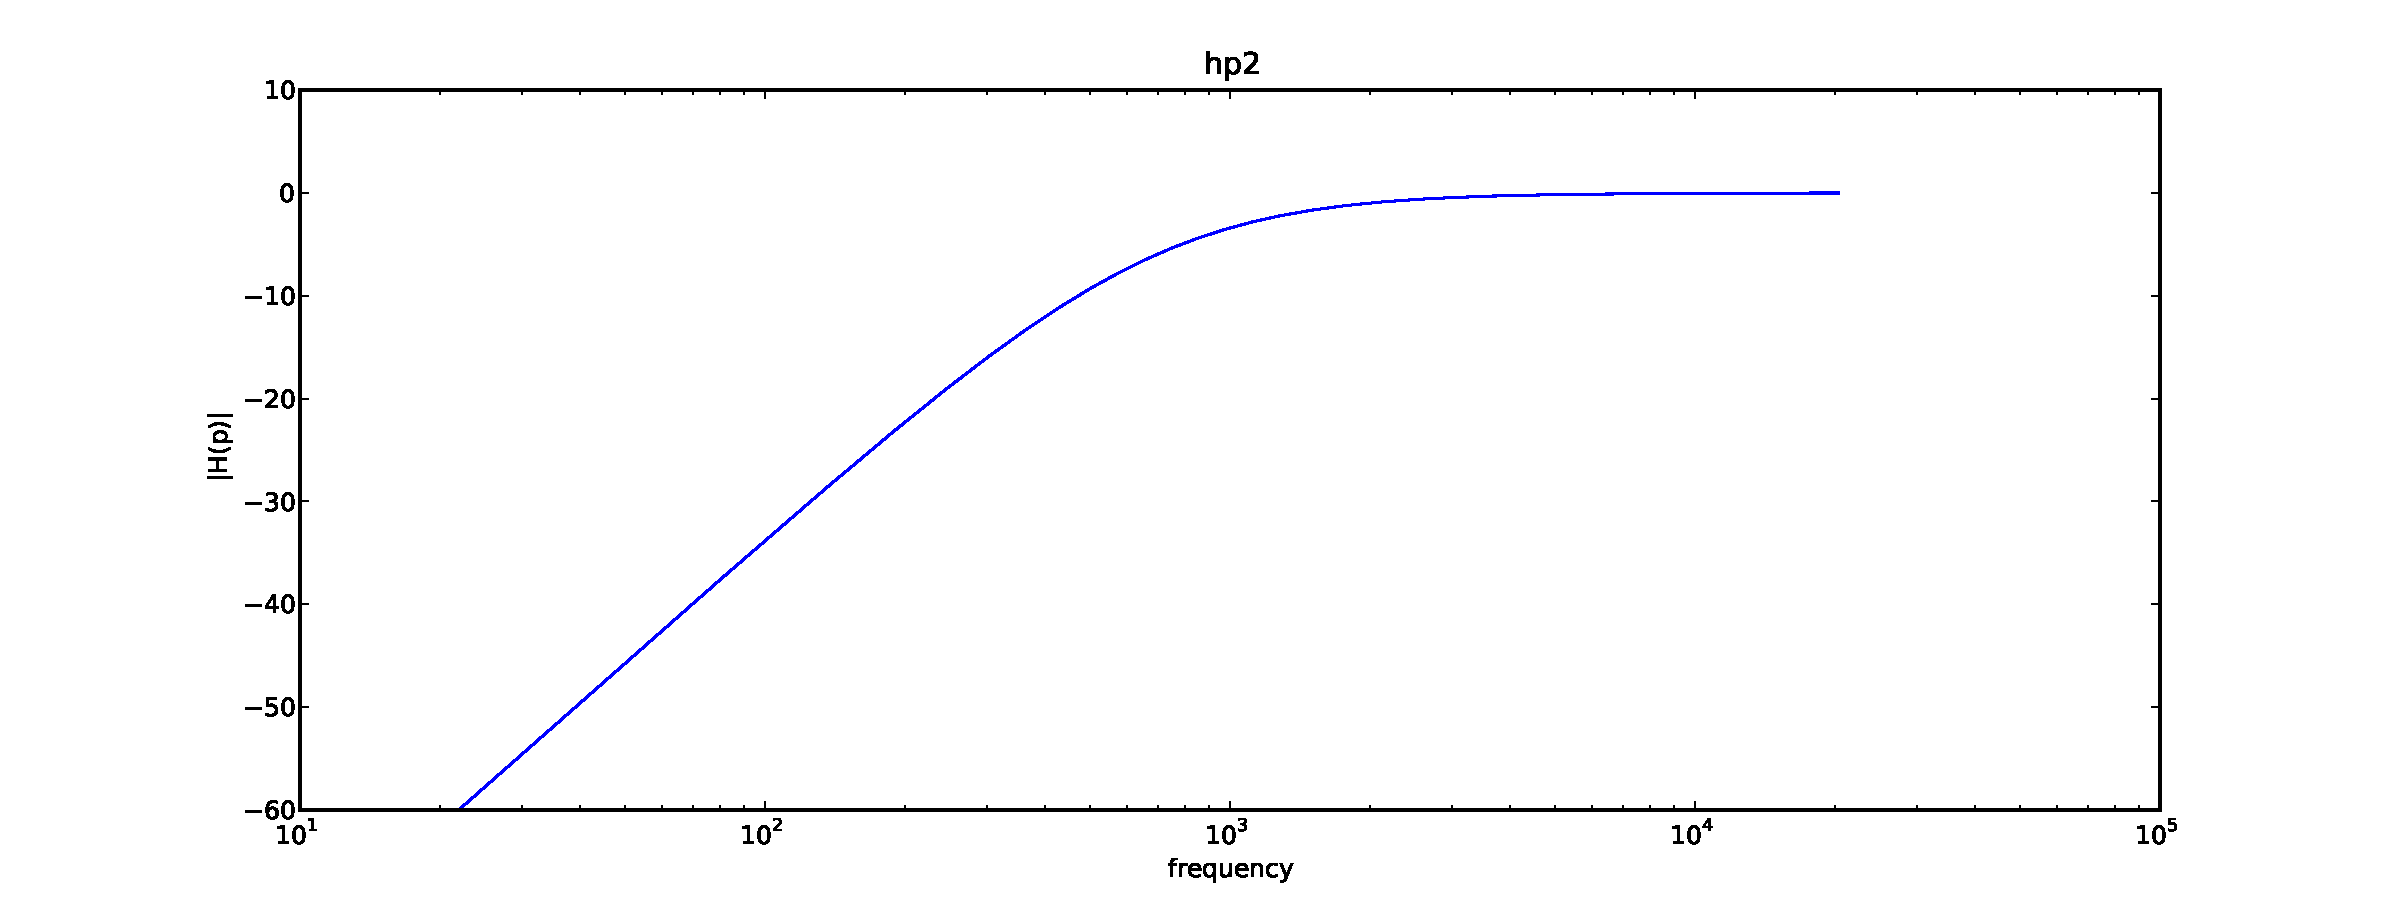
\includegraphics[width=0.4\textwidth]{response_hp2.pdf} & $\frac{s^2}{(1 + s)^2}$ & 1 & 2 & 1 & 0 & Disabled \\
\hline
HP3 & 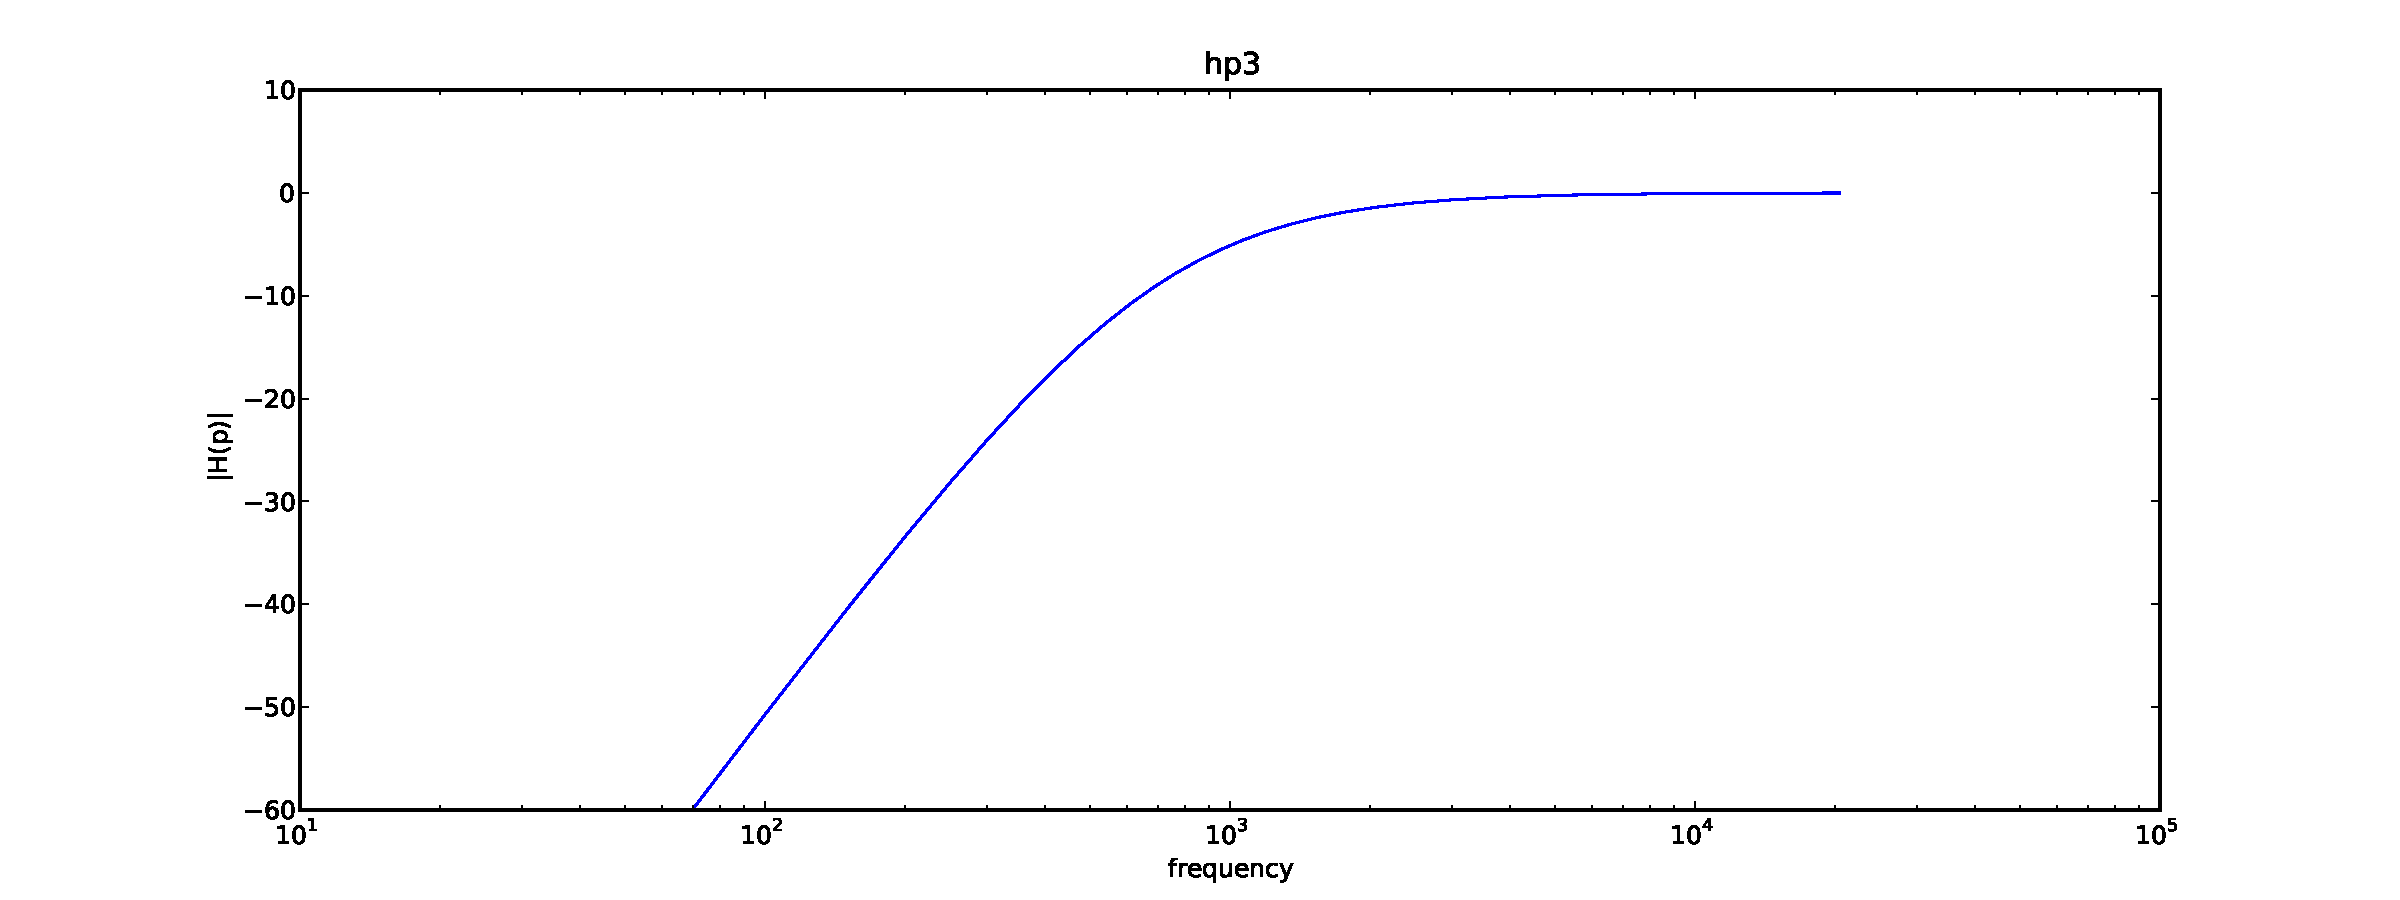
\includegraphics[width=0.4\textwidth]{response_hp3.pdf} & $\frac{s^3}{(1 + s)^3}$ & 1 & 3 & 3 & 1 & Disabled \\
\hline
\end{tabular}

\subsection{Band-pass modes}

\begin{tabular}{lcclllll}
\hline
Name & Response & Transfer function & $a$ & $b$ & $c$ & $d$ & First LP stage \\
\hline
BP2 & 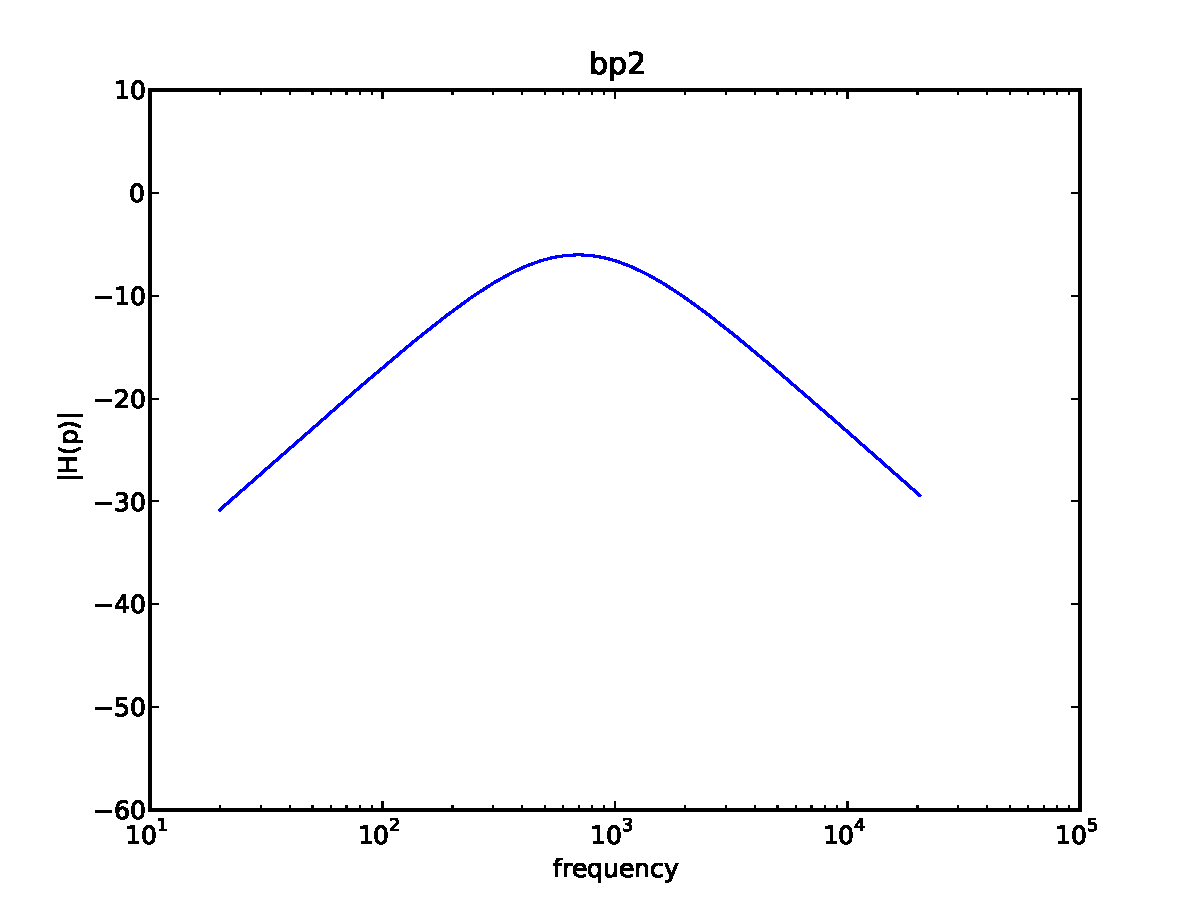
\includegraphics[width=0.4\textwidth]{response_bp2.pdf} & $\frac{s}{(1 + s)^2}$ & 1 & 1 & 0 & 0 & Enabled \\
\hline
BP4 & 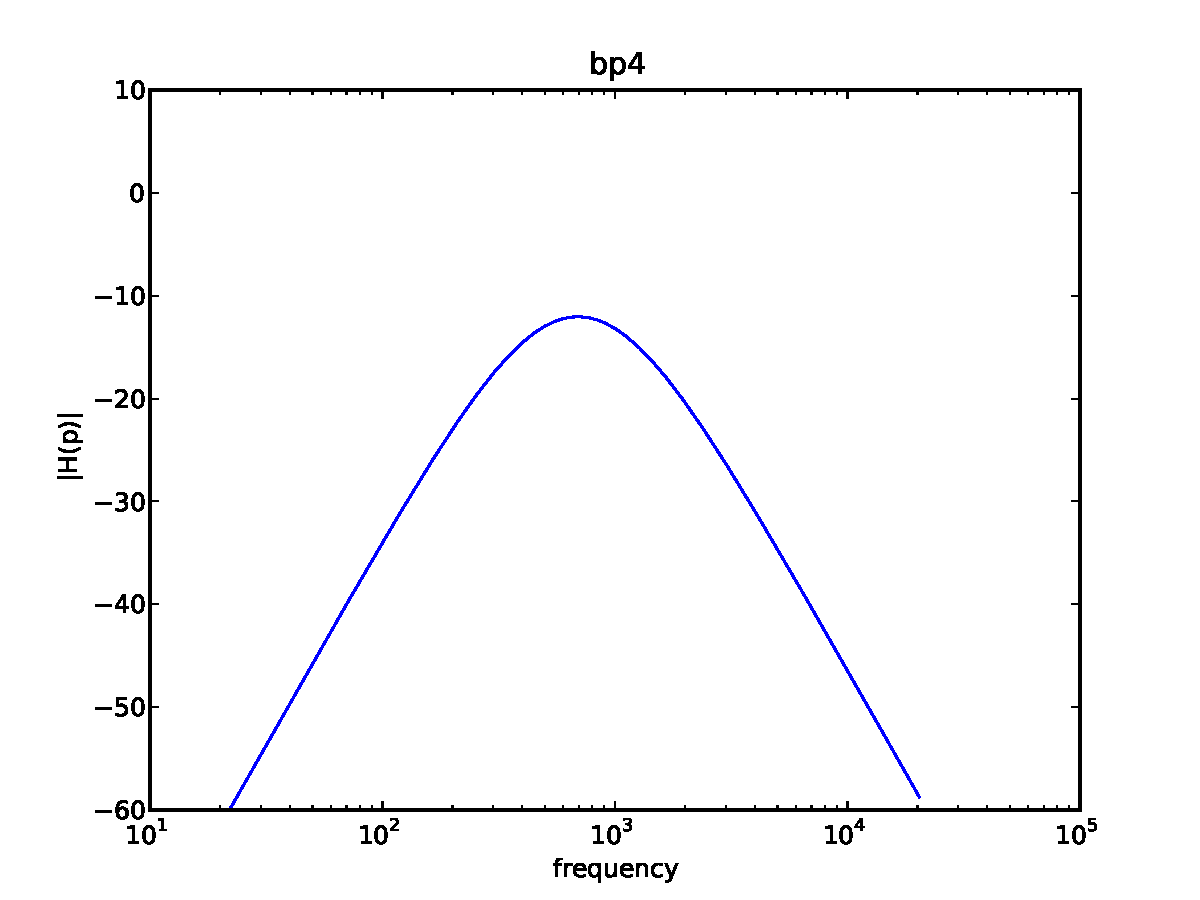
\includegraphics[width=0.4\textwidth]{response_bp4.pdf} & $\frac{s^2}{(1 + s)^4}$ & 0 & 1 & 2 & 1 & Enabled \\
\hline
\end{tabular}

\subsection{Notch and phaser modes}

\begin{tabular}{lcclllll}
\hline
Name & Response & Transfer function & $a$ & $b$ & $c$ & $d$ & First LP stage \\
\hline
Notch & 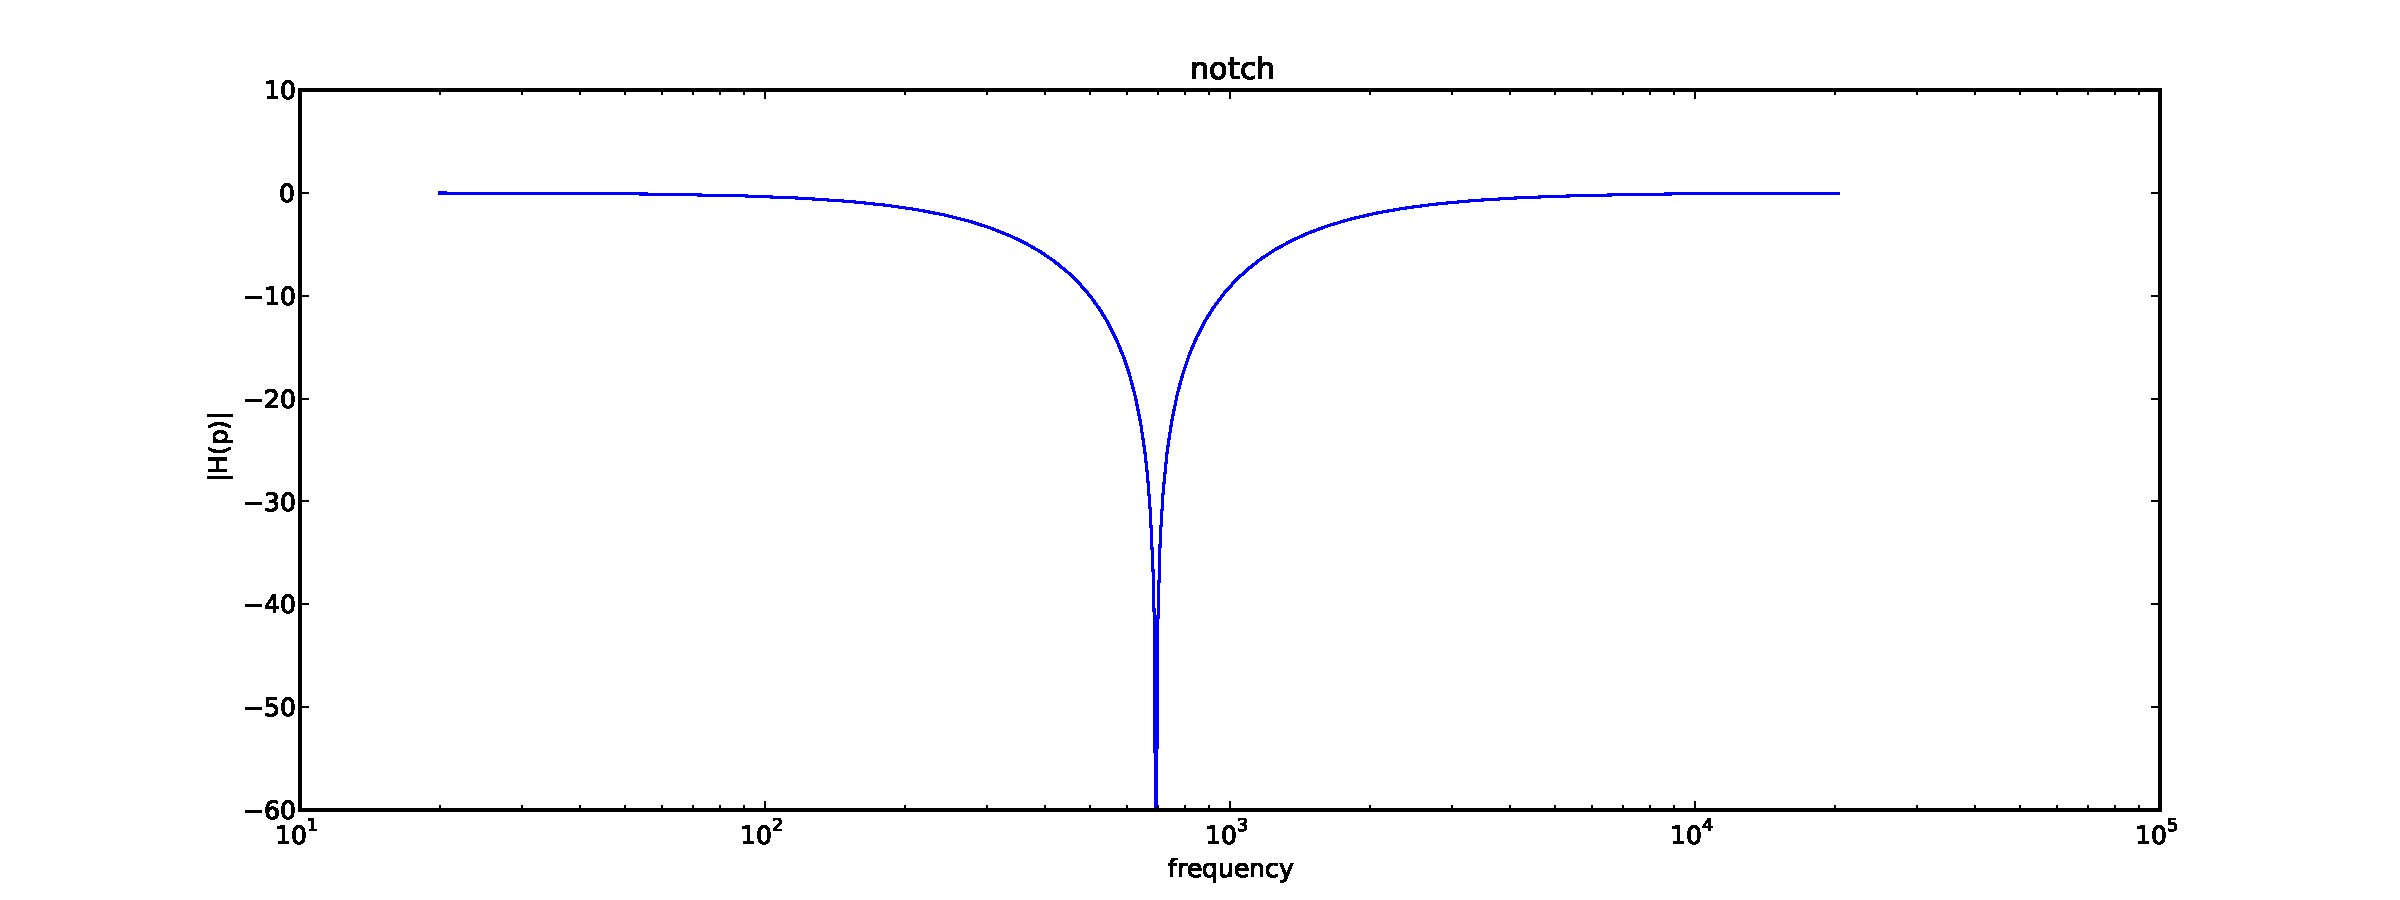
\includegraphics[width=0.4\textwidth]{response_notch.pdf} & $\frac{s^3 + s^2 + s + 1}{(1 + s)^3}$ & 1 & 2 & 2 & 0 & Disabled \\
\hline
Phaser & 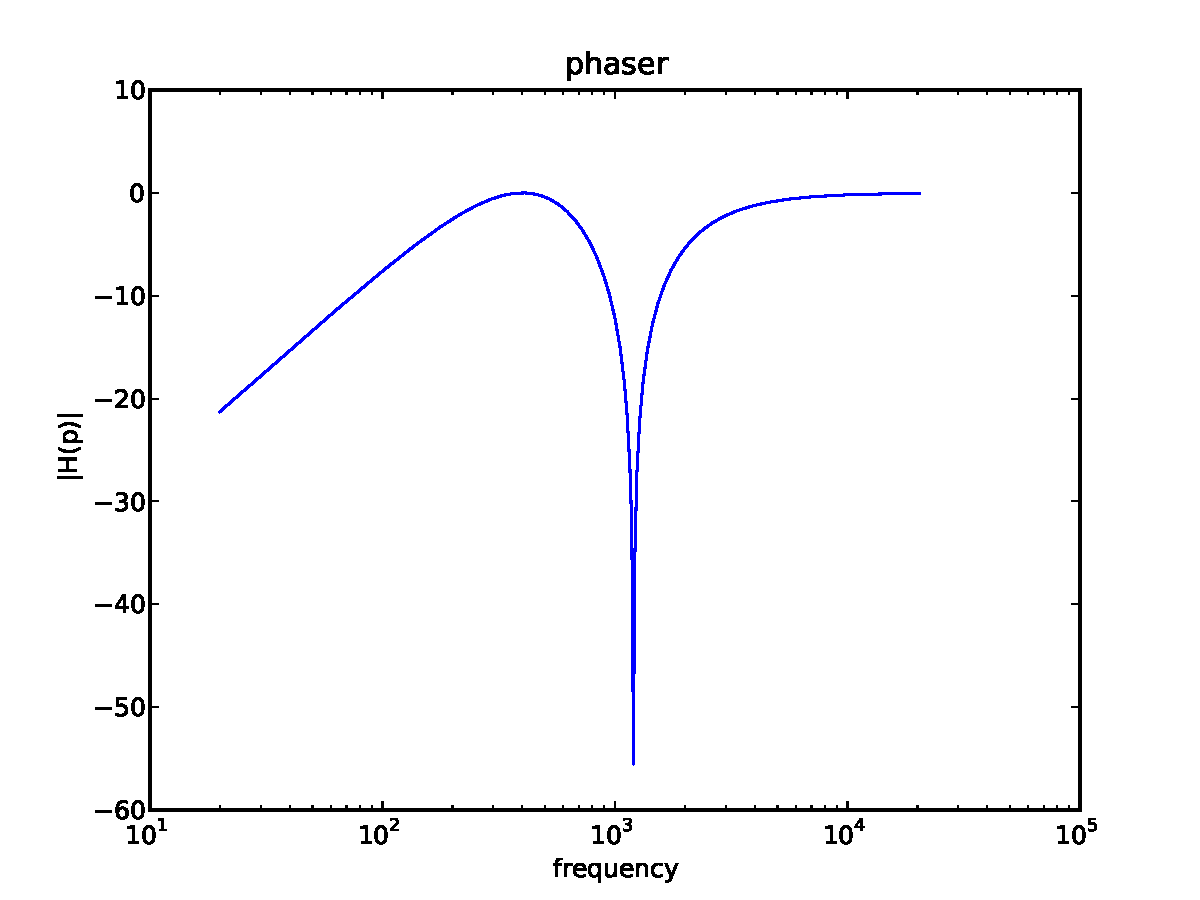
\includegraphics[width=0.4\textwidth]{response_phaser.pdf} & $1 - \frac{(1 - s)^3}{(1 + s)^3}$ & 1 & 3 & 6 & 4 & Disabled \\
\hline
\end{tabular}

\subsection{``Leftover" modes}

These modes are of little interest, but are cheap to realize by toggling the LP stage on already existing modes.

\begin{tabular}{lcclllll}
\hline
Name & Response & Transfer function & $a$ & $b$ & $c$ & $d$ & First LP stage \\
\hline
HP2 + LP1 & 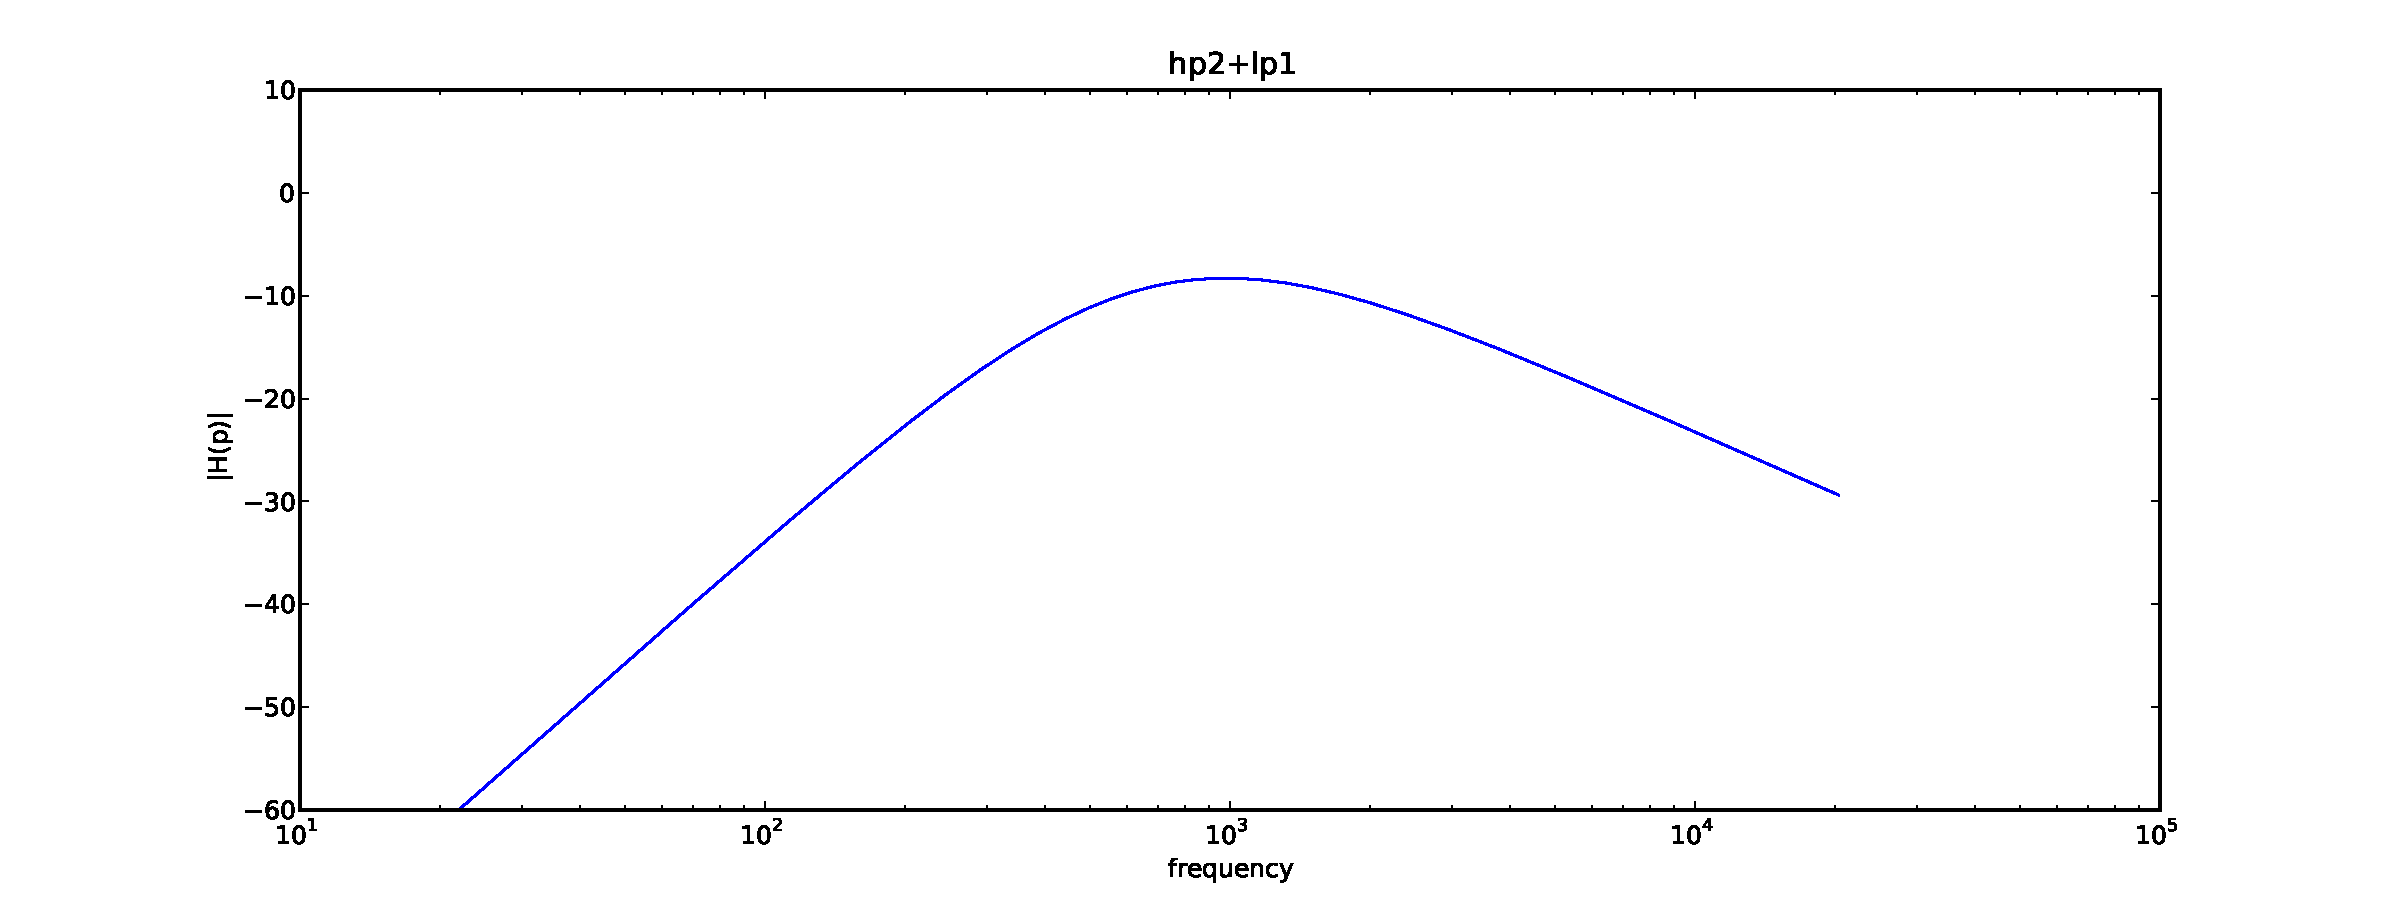
\includegraphics[width=0.4\textwidth]{response_hp2_lp1.pdf} & $\frac{s^3 + s^2}{(1 + s)^4}$ & 1 & 2 & 1 & 0 & Enabled \\
 & & & 0 & 1 & 2 & 1 & Disabled \\
\hline
HP3 + LP1 & 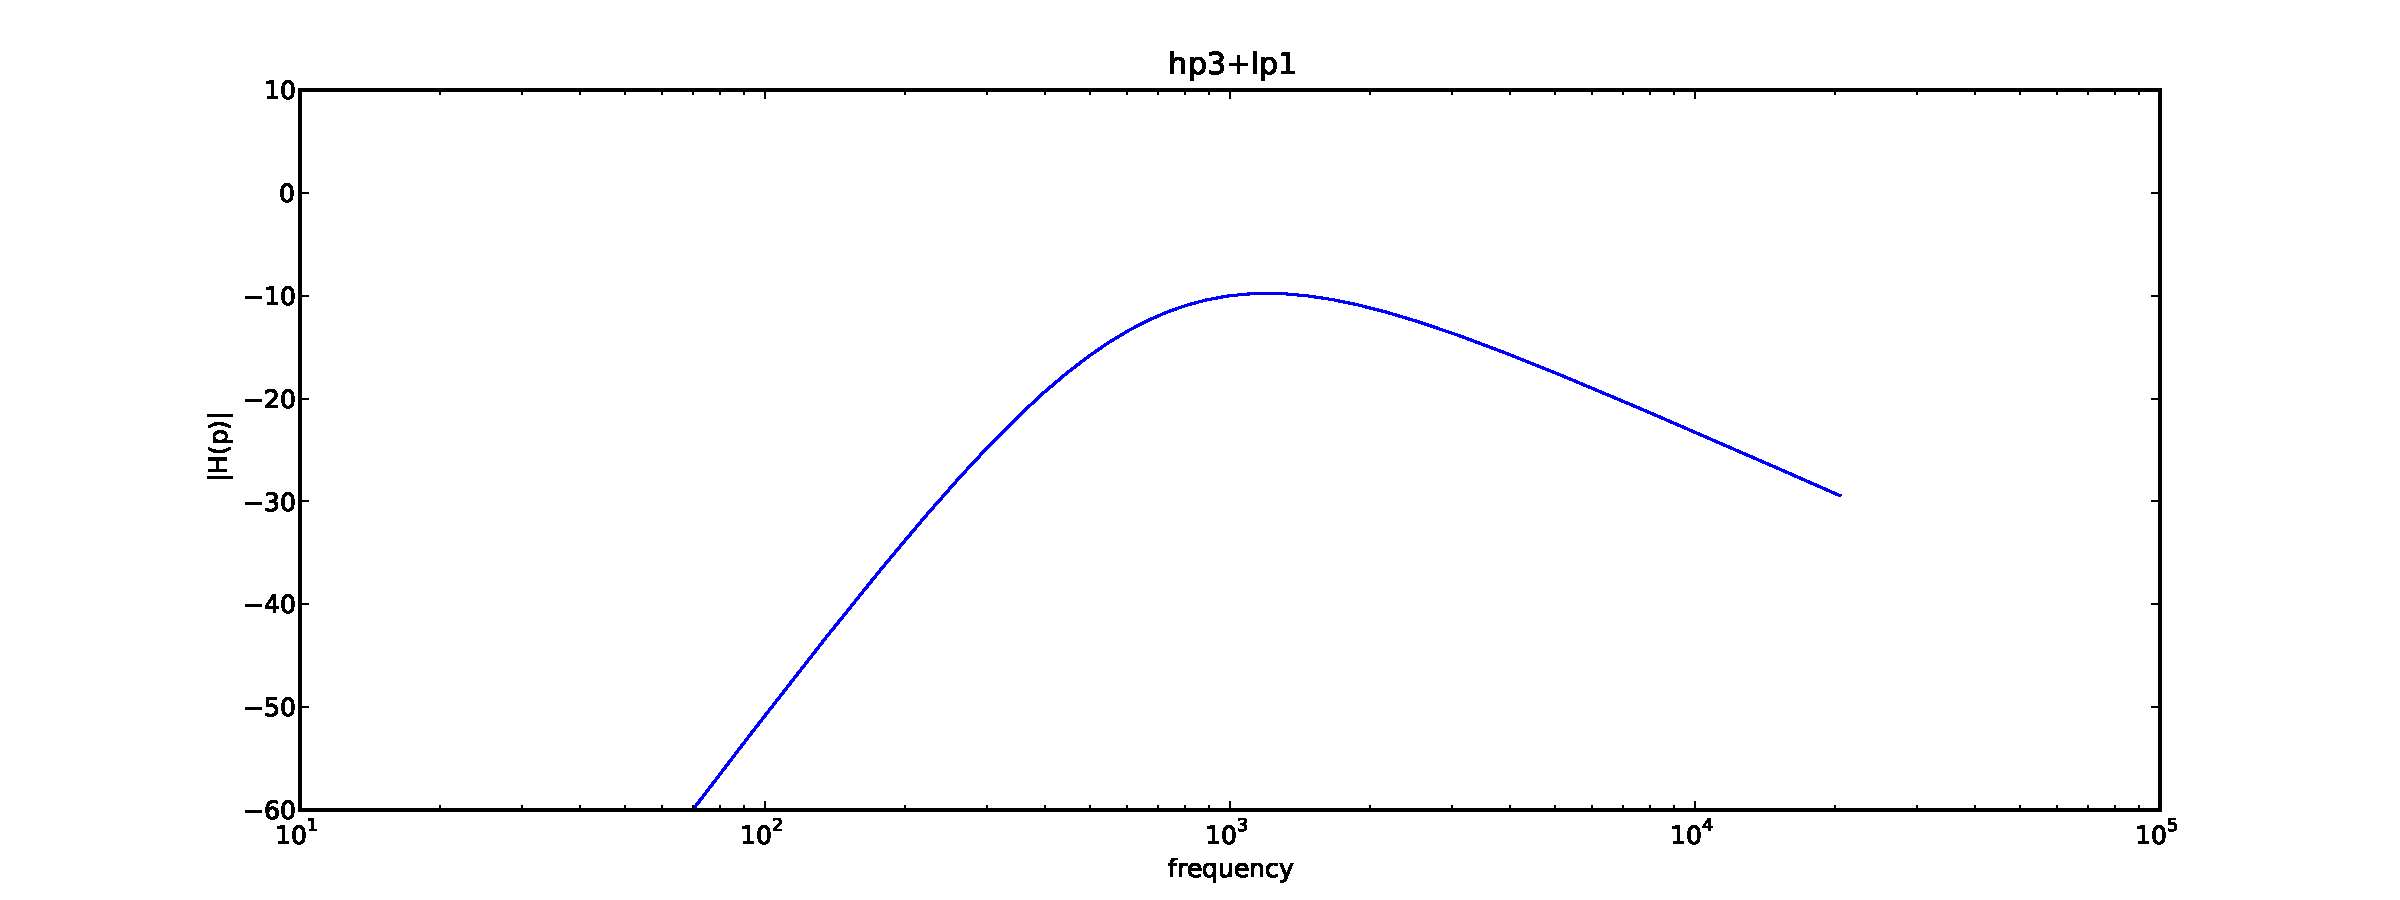
\includegraphics[width=0.4\textwidth]{response_hp3_lp1.pdf} & $\frac{s}{(1 + s)^4}$ & 1 & 3 & 3 & 1 & Enabled \\
\hline
Notch + LP1 & 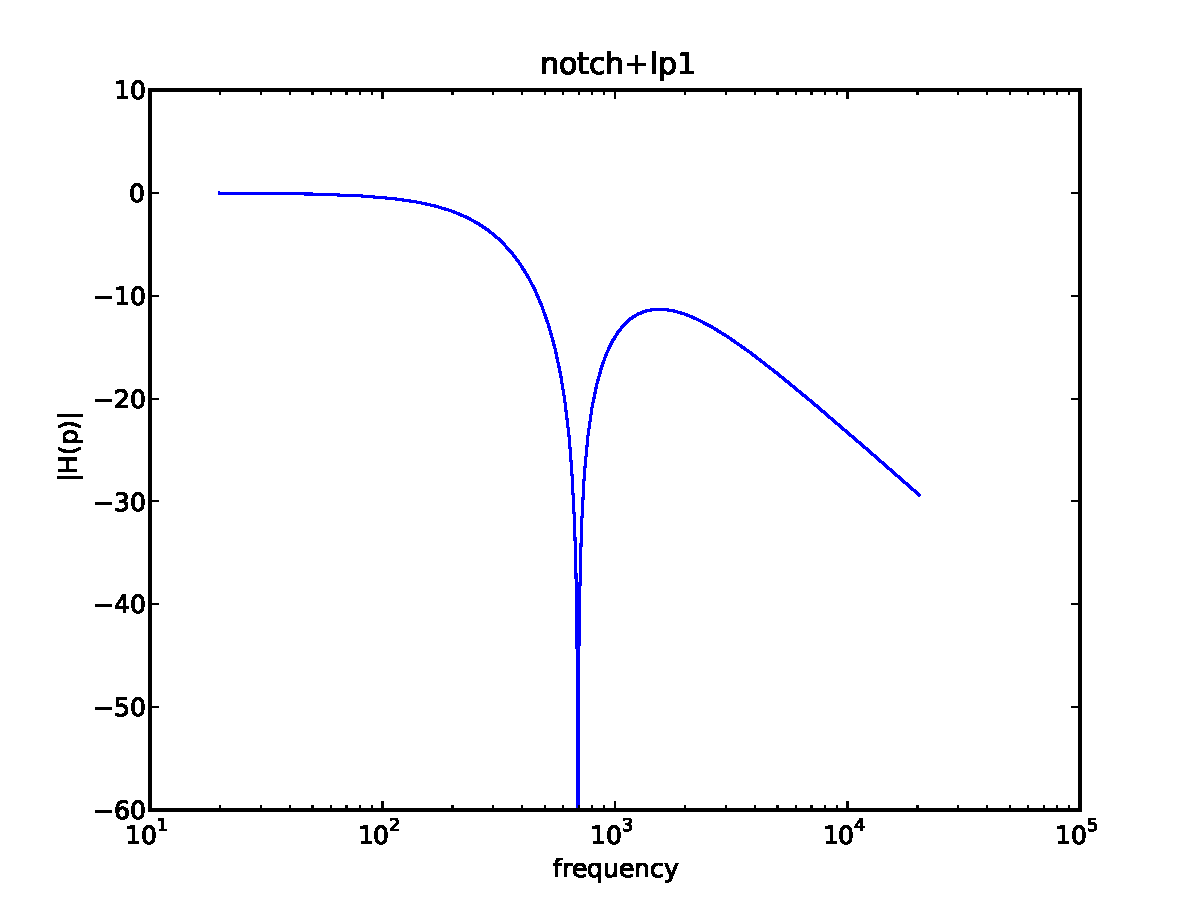
\includegraphics[width=0.4\textwidth]{response_notch_lp1.pdf} & $\frac{s^3 + s^2 + s + 1}{(1 + s)^4}$ & 1 & 2 & 2 & 0 & Enabled \\
\hline
Phaser + LP1 & 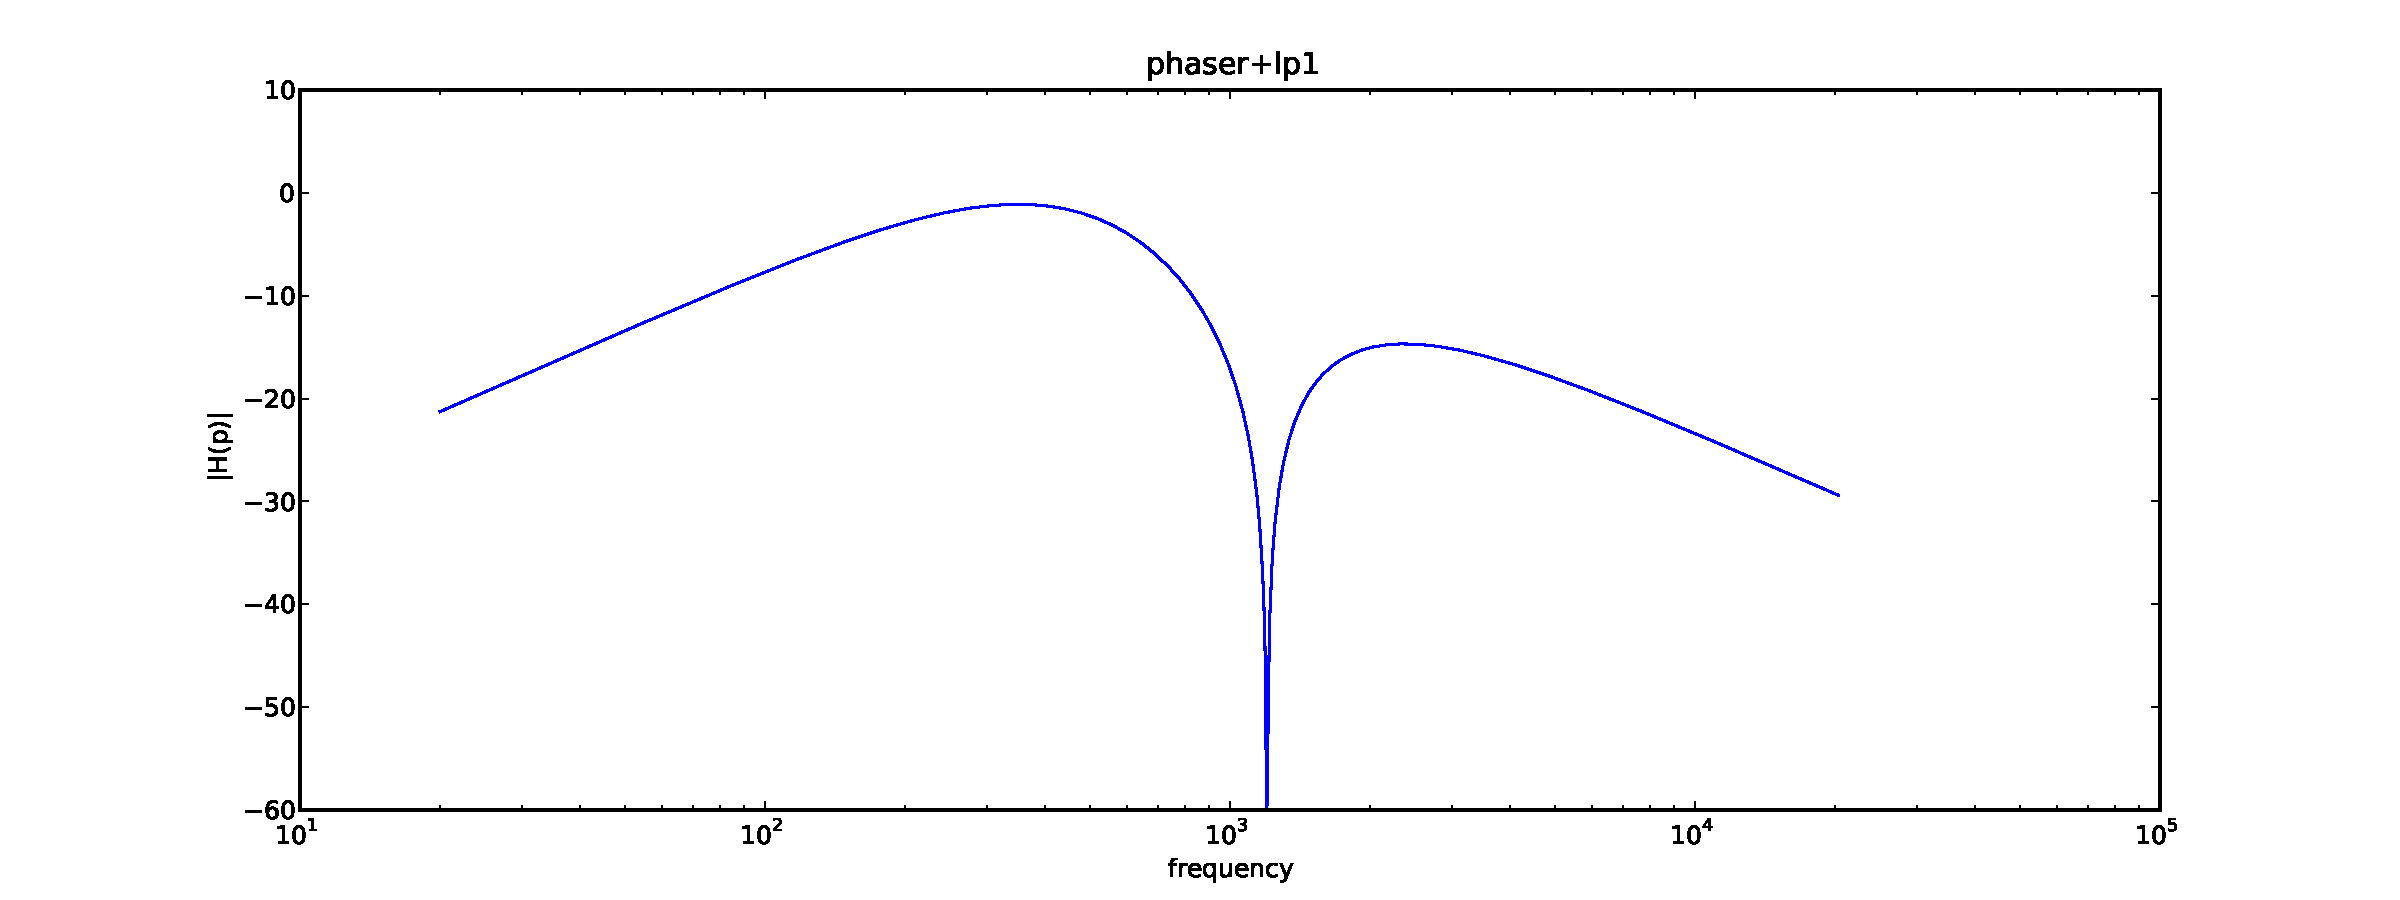
\includegraphics[width=0.4\textwidth]{response_phaser_lp1.pdf} & $\frac{1}{1 + s} - \frac{(1 - s)^3}{(1 + s)^4}$ & 1 & 3 & 6 & 4 & Enabled \\
\hline
\end{tabular}

\end{document}
